\documentclass[12pt,a4paper]{article}
\usepackage[utf8]{inputenc}
\usepackage[T1]{fontenc}
\usepackage{times}
\usepackage[margin=2.5cm]{geometry}
\usepackage{setspace}
\onehalfspacing
\usepackage{graphicx}
\usepackage{booktabs}
\usepackage{hyperref}
\usepackage{amsmath}

\title{Temples Without Villages: Candi and the Hidden Settlement Geography of Volcanic Java}

\author{Mukhlis Amien\textsuperscript{1} \and Go Frendi Gunawan\textsuperscript{1}}

\date{}

\begin{document}

\maketitle

\noindent\textsuperscript{1}Lab Data Sains, Universitas Bhinneka Nusantara, Malang, Indonesia

\vspace{0.5em}
\noindent\textbf{Corresponding author:} Mukhlis Amien (\texttt{amien@ubhinus.ac.id})\\
\noindent ORCID: 0000-0002-1848-167X

\begin{abstract}
Java's volcanic landscape has buried centuries of human settlement beneath metres of pyroclastic debris. We argue that surviving Hindu-Buddhist temples (\emph{candi}) mark the locations of these lost communities. Spatial analysis of 142 candi reveals systematic clustering on western volcanic flanks---precisely the zones most intensely buried---while temple \emph{orientation} follows religious prescription, demonstrating intentional landscape reading by their builders. Comparison with georeferenced inscriptions confirms that this volcanic proximity is specific to sacred architecture, not general settlement geography. The 2008 discovery of a complete buried village at Liangan validates the model. What emerges is a picture of pre-modern Java far more extensively settled than the surviving record suggests---a cultural landscape rendered invisible not by absence, but by geological process.
\end{abstract}

\vspace{0.5em}
\noindent\textbf{Keywords:} Java, candi, volcanic taphonomy, settlement geography, inscriptions, Hindu-Buddhist archaeology, Insulindia, buried landscapes

\newpage

% ============================================================
\section{Introduction: What Survives and What is Lost}
% ============================================================

The scholarly understanding of pre-modern Java rests on what the island's volcanic landscape has permitted to survive. Lombard's magisterial portrait of the ``Javanese crossroads'' drew upon inscriptions, temple complexes, and literary texts---all products of elite patronage, all rendered in durable media.\footnote{Denys Lombard, \emph{Le carrefour javanais: essai d'histoire globale}, 3 vols. (Paris: \'{E}ditions de l'\'{E}cole des hautes \'{e}tudes en sciences sociales, 1990).} Yet the villages, markets, workshops, and domestic spaces that constituted the lived experience of the vast majority of Javanese---built in wood, bamboo, and thatch---have left almost no archaeological trace. This is not because they did not exist, but because Java's 34 active volcanoes have been burying them at measurable rates for millennia.

The result is a historical record shaped as much by geological process as by human action. When Wolters described the ``localization'' of Indic culture in Southeast Asia, he worked primarily from inscriptions and temples---the very sources most likely to survive volcanic sedimentation.\footnote{O. W. Wolters, \emph{History, Culture, and Region in Southeast Asian Perspectives}, rev. ed. (Ithaca: Cornell University Southeast Asia Program, 1999).} The domestic, vernacular, and pre-Indic layers of Javanese civilization, by contrast, have been systematically removed from the evidential base. Miksic has noted the paradox: Java's archaeological record is simultaneously one of the richest in Southeast Asia (in monumental terms) and one of the most incomplete (in settlement terms).\footnote{John N. Miksic, ``The Classical Cultures of Indonesia,'' in \emph{Southeast Asia: From Prehistory to History}, ed. Ian Glover and Peter Bellwood (London: RoutledgeCurzon, 2004), 234--256.}

This paper proposes that surviving candi can serve as witnesses---not merely to the religious life of Hindu-Buddhist Java, but to the geography of an entire buried settlement landscape. By analysing where temples were built (and where they were not), we extract spatial information about past communities that no surface survey can now recover.

% ============================================================
\section{The Volcanic Landscape as Taphonomic Agent}
% ============================================================

Java hosts 34 of Indonesia's 127 active volcanoes, erupting on average once every 1--2 years.\footnote{Global Volcanism Program, \emph{Volcanoes of the World}, v. 5.1.1 (Smithsonian Institution, 2023), \url{https://volcano.si.edu/}.} Each eruption deposits pyroclastic material, lahars, and tephra that incrementally bury the surrounding landscape. Measured sedimentation rates at archaeological sites in East Java range from 3.6~mm/yr on distal plains to 13.1~mm/yr on proximal volcanic flanks.\footnote{Franck Lavigne and Jean-Claude Thouret, ``Sediment Transportation and Deposition by Rain-Triggered Lahars at Merapi Volcano, Central Java, Indonesia,'' \emph{Geomorphology} 49, no. 1--2 (2003): 45--69.}

Colonial-era archaeologists documented the consequences directly. The \emph{Oudheidkundig Verslag} reports of 1912--1929 record 24 instances of archaeological structures found at depth: a Vi\d{s}\d{n}u statue at Prambanan at 9.14~m below the modern surface, Trowulan structures at 3.5--4.3~m, temples near Kelud under 2~m of lahar deposit.\footnote{E. C. J. Mohr, ``The Relation between Soil and Population Density in the Netherlands East Indies,'' in \emph{Comptes Rendus du Congr\`{e}s International de G\'{e}ographie} (Amsterdam, 1938).} These depths render sites invisible to surface survey---the standard method of archaeological prospection in Indonesia.

The taphonomic process is not random. It preferentially erases evidence from the zones closest to volcanoes: the very areas that, in Mohr's analysis, supported the highest population densities due to the exceptional fertility of volcanic soils. The irony is precise: the geological process that made Java one of the most agriculturally productive islands in the world has simultaneously buried the archaeological evidence of the civilisations that productivity sustained.

% ============================================================
\section{What the Temples Show}
% ============================================================

\subsection{Candi as Survivors}

Hindu-Buddhist candi---monumental structures of andesite and brick---resist volcanic burial and tropical weathering far better than organic-material settlements. Of the 142 candi for which we compiled coordinates from published surveys, heritage registries, and Dumar\c{c}ay's and Soekmono's standard catalogues,\footnote{Jacques Dumar\c{c}ay, \emph{The Temples of Java} (Oxford: Oxford University Press, 1993). R. Soekmono, \emph{The Javanese Candi: Function and Meaning} (Leiden: Brill, 1995).} all were either continuously visible or rediscovered during colonial-era earthworks. They are, in Schiffer's terminology, products of differential formation processes: what survives is what resists.\footnote{Michael B. Schiffer, \emph{Formation Processes of the Archaeological Record} (Albuquerque: University of New Mexico Press, 1987).}

But candi were never isolated monuments. Each was the centre of a functioning community. Soekmono's study of candi function emphasised their role within settlement complexes---surrounded by villages, irrigated fields, markets, and craft production areas. The question, then, is what their spatial distribution can tell us about the communities that built them.

\subsection{Western Flanks, Volcanic Proximity}

Analysis of the bearing from each candi to its nearest active volcano reveals a striking pattern (Figure~\ref{fig:polar}). Mean bearing: 279\textdegree{} (west). Rayleigh test for circular non-uniformity: $p = 3.4 \times 10^{-8}$. Nearly half of all candi (47.2\%) lie on the western flanks of volcanoes; the eastern quadrant contains fewer than 4\%.

\begin{figure}[h]
\centering
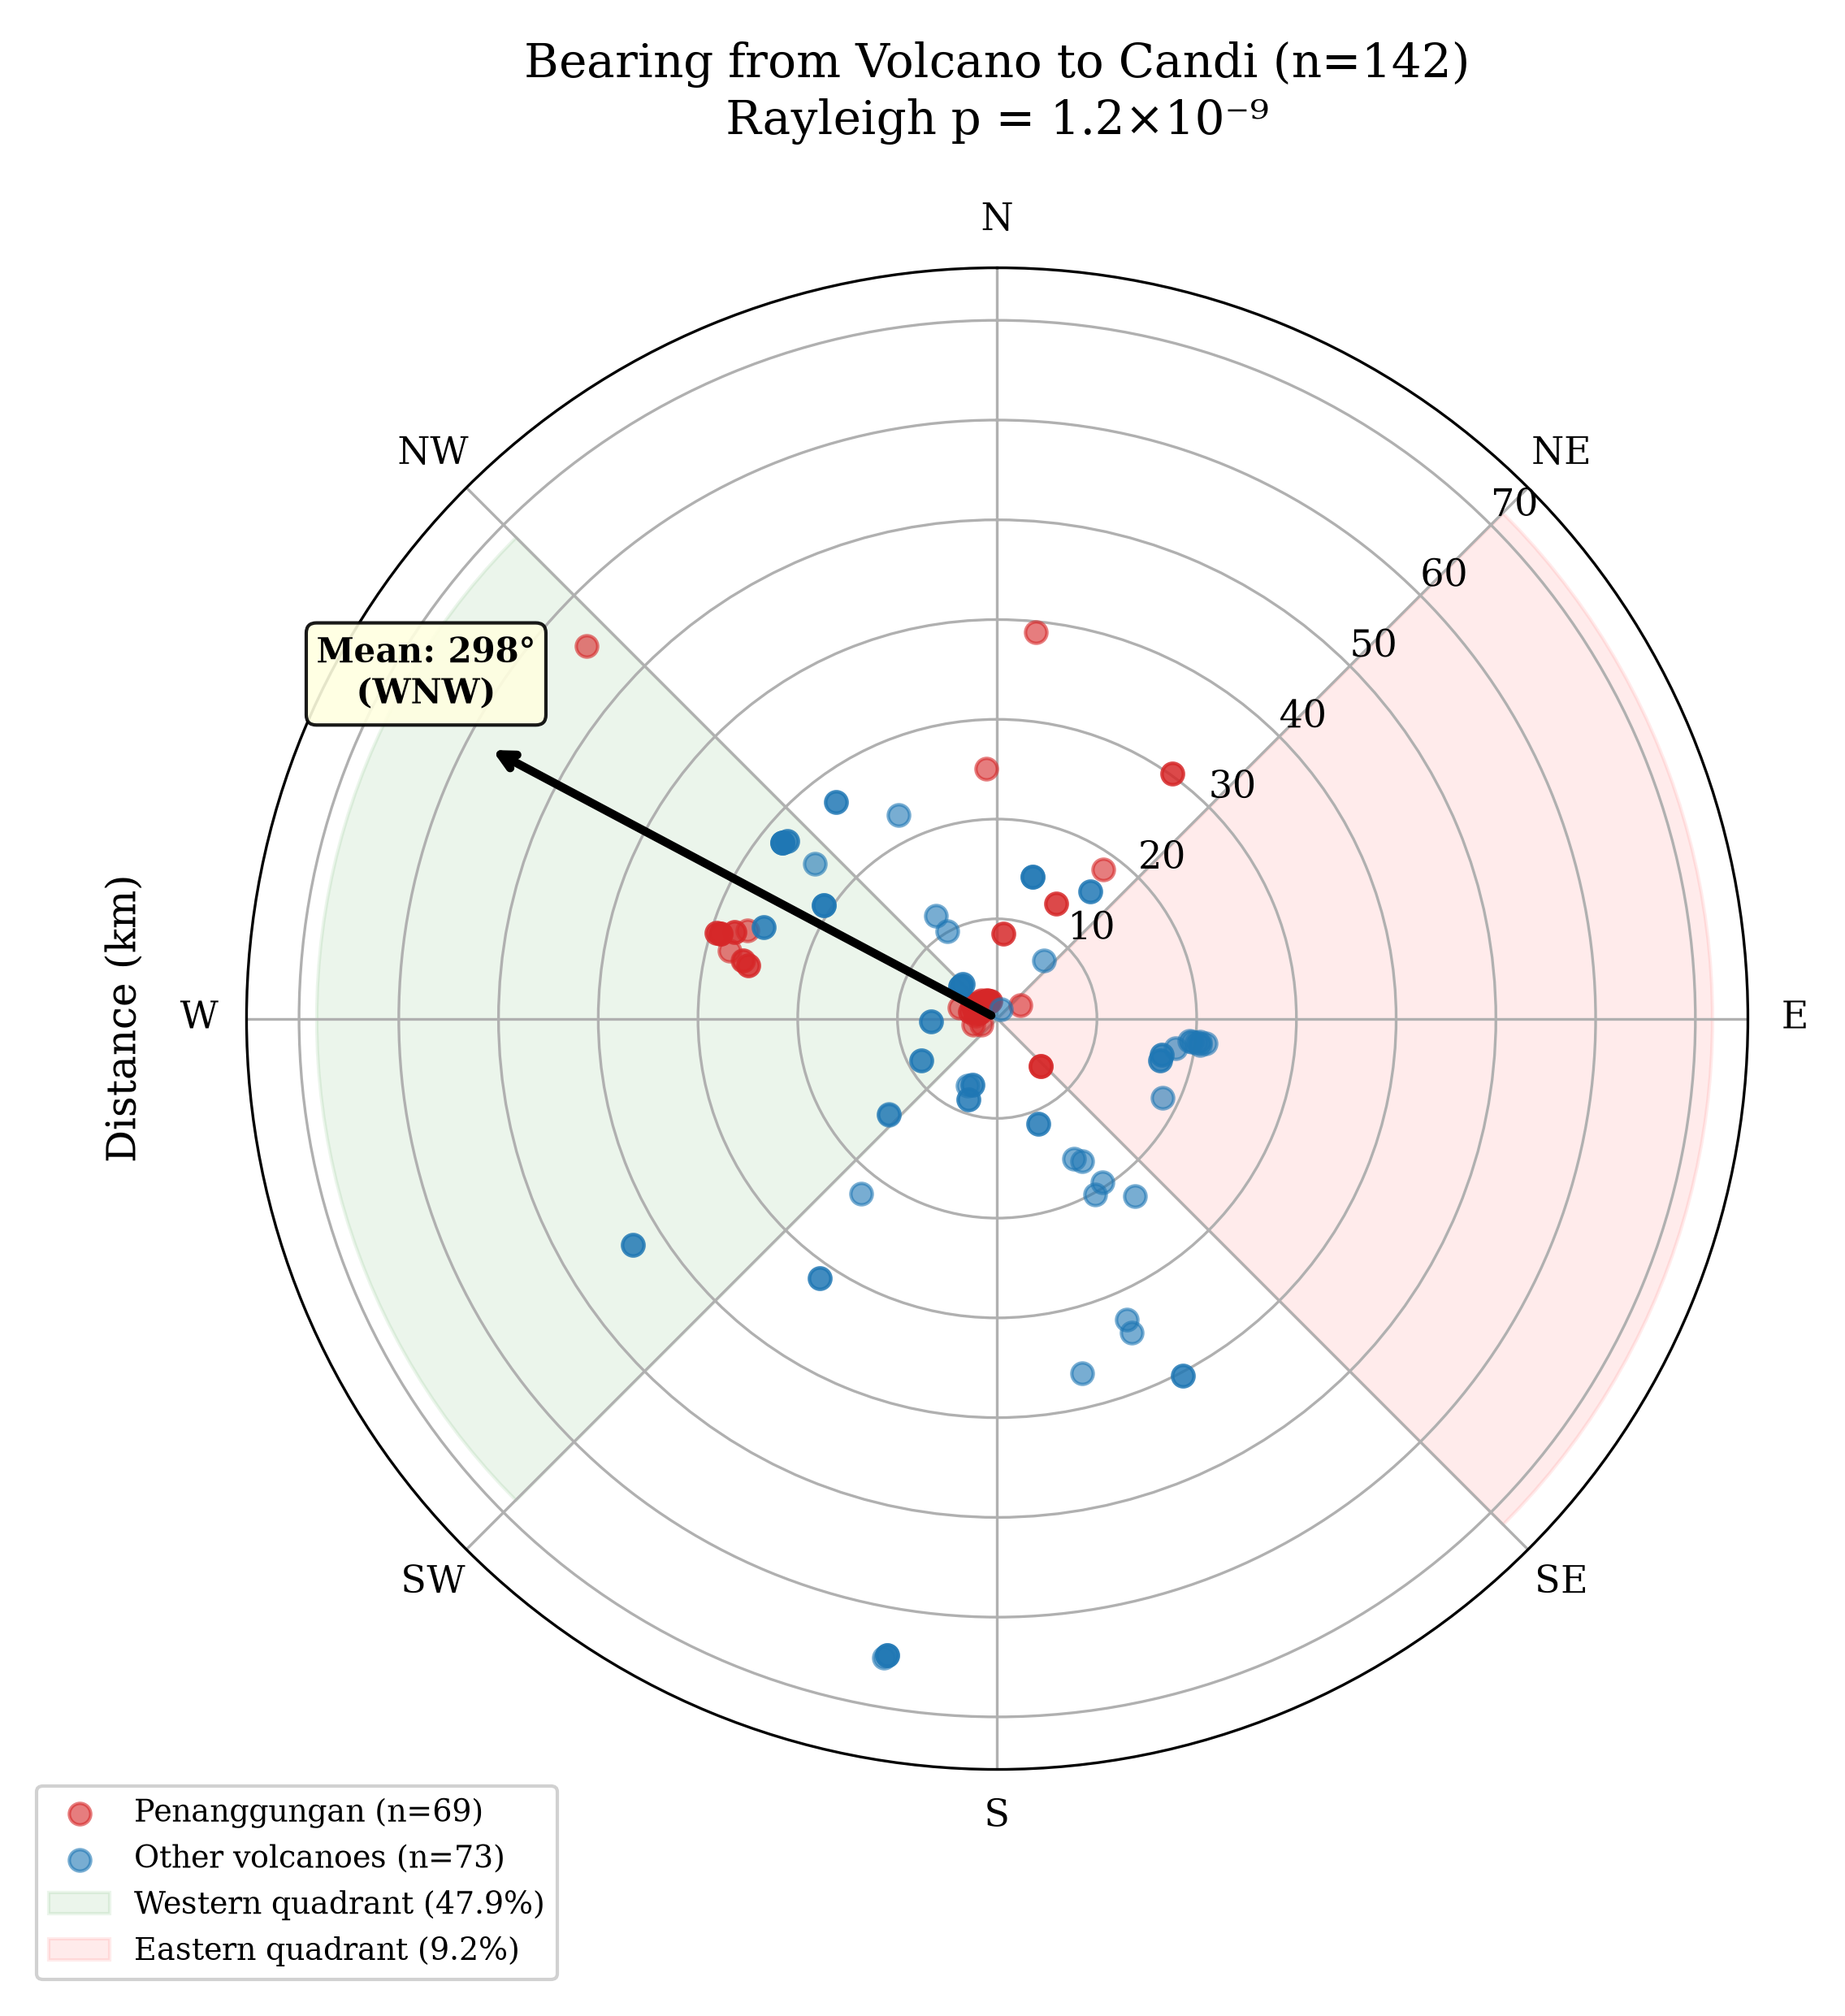
\includegraphics[width=0.7\textwidth]{figures/fig1_candi_polar_bearings.png}
\caption{Polar plot of candi bearings from nearest volcanic peak. The western clustering (mean 279\textdegree{}) is consistent with deliberate positioning on the leeward side of prevailing eruption plumes, where tephra deposition is minimised.}
\label{fig:polar}
\end{figure}

The proximity pattern is equally revealing. Zone A (within 10~km of a volcanic peak) contains 42.3\% of all candi---an overrepresentation of 17.9$\times$ relative to the proportion of land area in that zone. Zone C (beyond 30~km) is dramatically underrepresented at 0.15$\times$ expected.

\begin{table}[h]
\centering
\caption{Candi distribution across volcanic proximity zones}
\small
\begin{tabular}{lrrrr}
\toprule
Zone & Observed & Expected & Ratio & Interpretation \\
\midrule
A ($<$10 km) & 60 (42.3\%) & 3.4 & 17.9$\times$ & Densest past settlement \\
B (10--30 km) & 65 (45.8\%) & 27.0 & 2.4$\times$ & Substantial settlement \\
C ($>$30 km) & 17 (12.0\%) & 111.6 & 0.15$\times$ & Sparse settlement \\
\bottomrule
\end{tabular}
\label{tab:zones}
\end{table}

This is not driven by a single site. Penanggungan alone hosts 73 candi, 63\% on its western flank (Figure~\ref{fig:penanggungan}). But after excluding Penanggungan entirely, the remaining 69 candi across Java still show significant western clustering ($p = 0.0009$).

\begin{figure}[h]
\centering
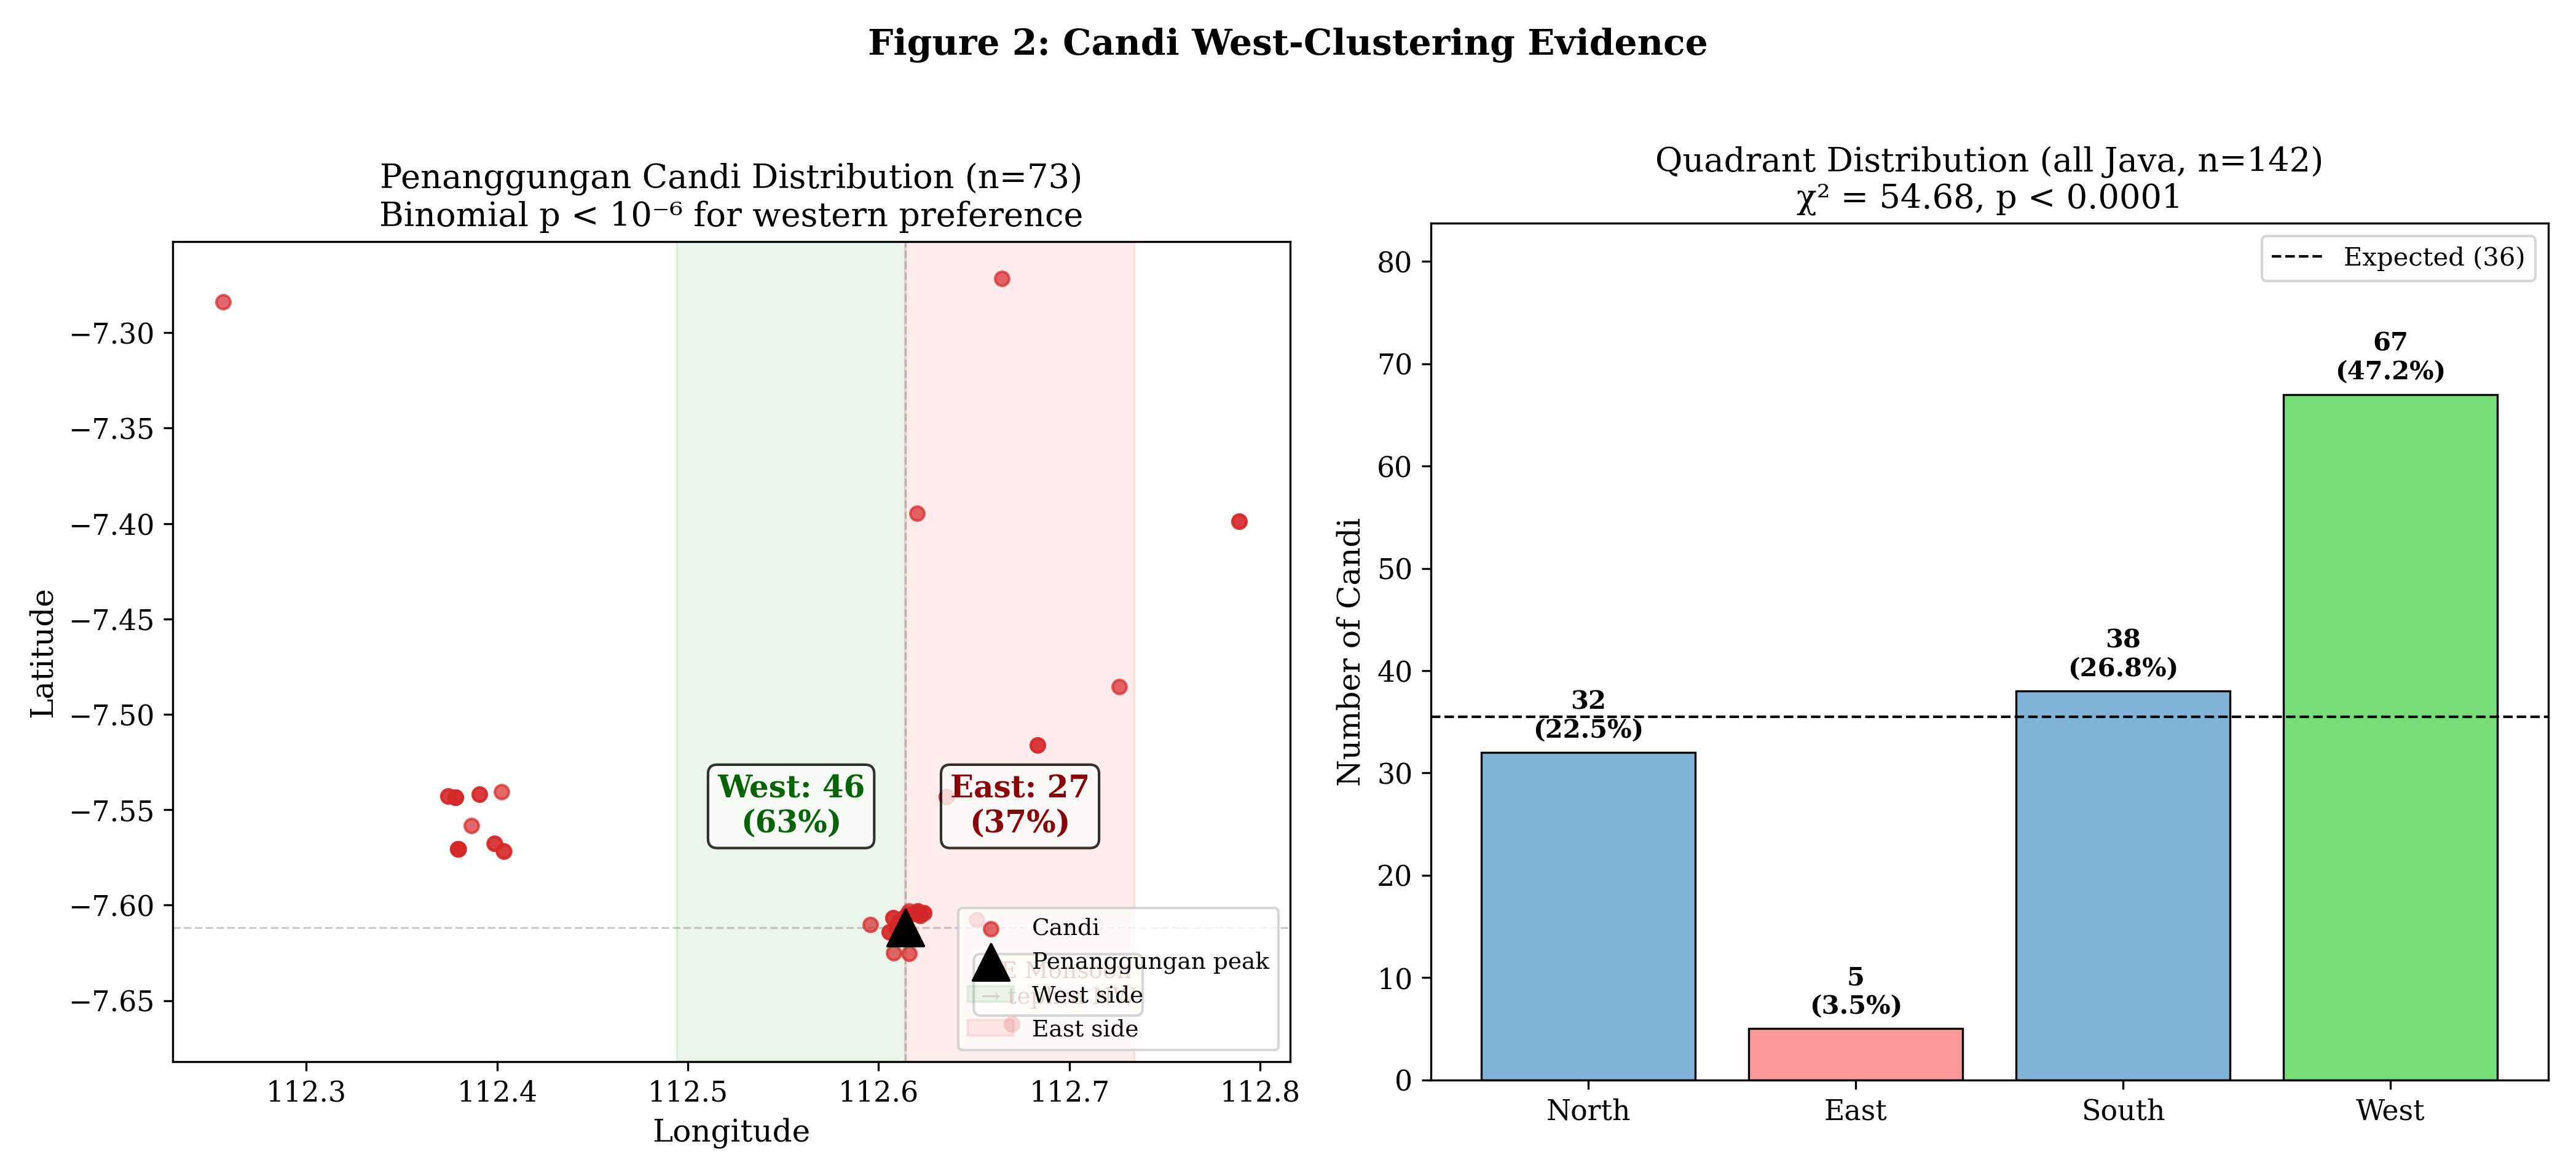
\includegraphics[width=0.7\textwidth]{figures/fig2_penanggungan_westclustering.png}
\caption{Distribution of 73 candi on Mount Penanggungan, showing the pronounced western-flank concentration. The pattern persists across Java after this mountain is excluded.}
\label{fig:penanggungan}
\end{figure}

\subsection{Orientation Follows Canon, Siting Follows Landscape}

A critical distinction emerges when we examine not where candi were placed but how they were oriented. Of 20 candi with documented entrance orientations, 85\% face the equinox direction (east or west; binomial $p = 4.9 \times 10^{-14}$), while only 35\% face toward the nearest volcano---indistinguishable from random expectation ($p = 0.94$).

The builders of Java's temples, in other words, simultaneously followed two distinct logics: a religious canon governing how temples should face, and a landscape-level understanding of volcanic geography governing where temples should stand. This intentionality is what makes the candi distribution informative---it is not random scatter, but a deliberate spatial record of where communities chose to build.

% ============================================================
\section{The Inscription Contrast}
% ============================================================

If candi proximity to volcanoes merely reflected general settlement geography, we would expect inscriptions---which record administrative activity across the inhabited landscape---to show a similar spatial distribution. We georeferenced 170 inscriptions from the DHARMA epigraphic database,\footnote{DHARMA project, \emph{The Domestication of ``Hindu'' Asceticism and the Religious Making of South and Southeast Asia: Epigraphic Database} (CNRS/ERC, 2024), \url{https://dharma.hypotheses.org/}.} producing the first spatially resolved inscription dataset for the region.

The contrast is stark. Inscriptions are on average 9.2~km farther from volcanoes than candi (Mann-Whitney $p = 5.2 \times 10^{-8}$). While 42.3\% of candi lie in Zone A, only 12.9\% of inscriptions do.

\begin{table}[h]
\centering
\caption{Spatial distribution: candi vs.\ inscriptions relative to nearest active volcano}
\begin{tabular}{lrrrr}
\toprule
 & \multicolumn{2}{c}{Candi ($n=142$)} & \multicolumn{2}{c}{Inscriptions ($n=170$)} \\
\midrule
Zone & $n$ & \% & $n$ & \% \\
\midrule
A ($<$10 km) & 60 & 42.3 & 22 & 12.9 \\
B (10--30 km) & 65 & 45.8 & 111 & 65.3 \\
C ($>$30 km) & 17 & 12.0 & 37 & 21.8 \\
\midrule
Mean distance & \multicolumn{2}{c}{16.5 km} & \multicolumn{2}{c}{25.7 km} \\
\bottomrule
\end{tabular}
\label{tab:inscr_candi}
\end{table}

This divergence has a temporal dimension. Before the political migration from Central to East Java in 929~CE, inscriptions cluster at a mean of 16.2~km from volcanoes (reflecting proximity to Merapi). After 929, they shift to 38.4~km ($p = 5.3 \times 10^{-8}$). The architectural record, by contrast, maintains volcanic proximity across both periods---dominated in the east by Penanggungan (mean 7.4~km).

What this suggests is that the sacred landscape and the administrative landscape operated according to different spatial logics. Candi were placed close to volcanoes; the apparatus of the state, as recorded in inscriptions, operated at greater distance. The implication for understanding settlement geography is that temple locations reflect a layer of spatial information not captured by the epigraphic record alone.

% ============================================================
\section{Liangan: The Buried Village Revealed}
% ============================================================

The discovery of Liangan in 2008 provides direct validation. Located 5.5~km from Mount Sindoro on its western flank---Zone A, western quadrant---the site was found not by archaeologists but by sand miners, who exposed a complete Mataram-era settlement beneath 6--8~m of pyroclastic deposits.\footnote{Novida Abbas, ed., \emph{Liangan: Mozaik Peradaban Mataram Kuno di Lereng Sindoro} (Yogyakarta: Kepel Press / Balai Arkeologi Yogyakarta, 2016).}

What Liangan preserved is precisely what our analysis predicts should exist but cannot be detected: wooden houses, carbonised rice grains (\emph{tropical japonica}), iron-smelting workshops, Tang Dynasty ceramics, and the complete domestic infrastructure of a Hindu-Buddhist-era village. It is, in the Indonesian context, a Cer\'{e}n---the Central American village sealed by a single eruption c.~600 CE that preserved sleeping mats and food in vessels.\footnote{Payson D. Sheets, ed., \emph{Before the Volcano Erupted: The Ancient Cer\'{e}n Village in Central America} (Austin: University of Texas Press, 2002).}

Liangan is not an anomaly. It is a window. If the spatial patterns identified in this paper are correct, dozens of similar sites lie beneath the volcanic deposits of East Java's western flanks, awaiting discovery---or destruction by unmonitored mineral extraction.

% ============================================================
\section{The Question of Survey Investment}
% ============================================================

A potential objection is that the archaeological gap near volcanoes reflects differential survey effort rather than genuine burial. We tested this using an robustness regression controlling for three survey-intensity proxies (road distance, proximity to heritage offices, university proximity). After controlling for all three, volcanic proximity still explains additional variance in site counts ($p = 0.0015$). The volcanic-zone deficit is not solely a survey artifact.

The comparison with Japan sharpens this point. Japan hosts 111 active volcanoes and has one of the world's richest archaeological records in volcanic terrain---including settlements buried by Mount Haruna's 6th-century eruptions.\footnote{Satoru Shimoyama, ``Volcanic Disasters and Archaeological Sites in Southern Kyushu, Japan,'' in \emph{Natural Disasters and Cultural Change}, ed. Robin Torrence and John Grattan (London: Routledge, 2002), 326--341. Gina L. Barnes, ``Origins of the Japanese Islands: The New `Big Picture,'\,'' \emph{Japan Review} 15 (2003): 3--50.} But these sites were discovered through rescue archaeology---approximately 8,300 excavations per year, compared to Indonesia's approximately 70.\footnote{Hiroki Takata and Takahiro Yanase, ``Production, Preservation and Dissemination of Archaeological Data in Japan,'' \emph{Internet Archaeology} 58 (2022).} Japan has overcome the geological barrier through institutional investment. Indonesia has not.

The implication is not that Java is less historically rich than Japan. It is that the mechanisms by which buried sites become known---systematic rescue archaeology, developer-funded excavation, ground-penetrating radar surveys---have not been deployed at scale in Indonesia. What we cannot see is not what does not exist.

% ============================================================
\section{A Buried Cultural Landscape}
% ============================================================

The convergence of these evidence lines---candi clustering on western volcanic flanks, the inscription-architecture divergence, documented burial depths of 3--9~m, the Liangan discovery, and the survey-intensity test---points toward a single conclusion: pre-modern Java was far more extensively settled in volcanic zones than the surviving record indicates.

This has implications beyond archaeology. If the areas richest in surviving temples are also the areas where sedimentation has been most intense, then the monumental record we possess---the candi, the inscriptions, the literary texts---represents only the fraction of Javanese civilisation that happened to be encoded in durable media \emph{and} located at distances or depths where survival was possible. The vernacular layer---the houses, the markets, the workshops, the rice granaries---has been systematically subtracted from the evidential base.

Lombard's ``Javanese crossroads'' may therefore be not merely a crossroads but a buried crossroads, whose full extent remains to be excavated. The spatial patterns identified here suggest where recovery might begin: the western flanks of East Java's volcanoes, within 10~km of peaks, at depths of 3--13~m. Ten priority fieldwork targets derived from the intersection of candi clustering, terrain suitability, and sedimentation rate estimates are available upon request to authorised heritage bodies.

The candi-settlement proxy test strengthens this conclusion. Of 108 known non-temple archaeological sites in East Java, 81\% lie within 10~km of the nearest candi (mean distance 6.8~km; Monte Carlo $p < 0.0001$). Candi and settlements are spatially co-located, not independent---confirming that temples genuinely mark the centres of broader settlement complexes.

\subsection{Limitations}

The Penanggungan concentration (51\% of all candi) limits spatial generalisability, though the pattern survives its exclusion. All evidence remains indirect---no subsurface validation has yet been conducted. The temporal range of the candi proxy (c.~8th--15th century) does not extend to the pre-Hindu or Islamic periods, which require different evidential strategies.

% ============================================================
\section{Conclusion}
% ============================================================

The temples of Java stand as markers of a civilisation far larger than what survives. By reading their spatial distribution---not as a catalogue of monuments but as a map of past communities---we can begin to reconstruct the settlement geography that volcanic sedimentation has erased.

This is not merely a methodological contribution. It is a reframing of how we understand the archaeological record of the world's most volcanically active island. The silence in the record is not evidence of absence; it is evidence of burial. And the temples, paradoxically, are both survivors of that process and guides to what lies beneath.

% ============================================================
\subsection*{Data Availability}
% ============================================================

The candi coordinate dataset, georeferenced inscription dataset, tephra-archaeological correlation dataset, and all computational scripts are available at: \url{https://github.com/neimasilk/volcarch-repo}. GPS coordinates of predicted fieldwork targets are restricted to authorised heritage bodies (BPCB, Balai Arkeologi).

% ============================================================
\subsection*{AI Disclosure}
% ============================================================

This research used AI tools (Claude, Anthropic) for spatial geocoding, statistical computation, and manuscript drafting assistance. Research design, hypothesis formation, data interpretation, and all conclusions are the authors' work.

% ============================================================
\section*{Bibliography}
% ============================================================

\noindent Abbas, Novida, ed. \emph{Liangan: Mozaik Peradaban Mataram Kuno di Lereng Sindoro}. Yogyakarta: Kepel Press / Balai Arkeologi Yogyakarta, 2016.

\vspace{0.5em}
\noindent Barnes, Gina L. ``Origins of the Japanese Islands: The New `Big Picture.'\,'' \emph{Japan Review} 15 (2003): 3--50.

\vspace{0.5em}
\noindent DHARMA project. \emph{The Domestication of ``Hindu'' Asceticism and the Religious Making of South and Southeast Asia: Epigraphic Database}. CNRS/ERC, 2024. \url{https://dharma.hypotheses.org/}.

\vspace{0.5em}
\noindent Dumar\c{c}ay, Jacques. \emph{The Temples of Java}. Oxford: Oxford University Press, 1993.

\vspace{0.5em}
\noindent Global Volcanism Program. \emph{Volcanoes of the World}. V. 5.1.1. Smithsonian Institution, 2023. \url{https://volcano.si.edu/}.

\vspace{0.5em}
\noindent Lavigne, Franck, and Jean-Claude Thouret. ``Sediment Transportation and Deposition by Rain-Triggered Lahars at Merapi Volcano, Central Java, Indonesia.'' \emph{Geomorphology} 49, no. 1--2 (2003): 45--69.

\vspace{0.5em}
\noindent Lombard, Denys. \emph{Le carrefour javanais: essai d'histoire globale}. 3 vols. Paris: \'{E}ditions de l'\'{E}cole des hautes \'{e}tudes en sciences sociales, 1990.

\vspace{0.5em}
\noindent Miksic, John N. ``The Classical Cultures of Indonesia.'' In \emph{Southeast Asia: From Prehistory to History}, edited by Ian Glover and Peter Bellwood, 234--256. London: RoutledgeCurzon, 2004.

\vspace{0.5em}
\noindent Mohr, E. C. J. ``The Relation between Soil and Population Density in the Netherlands East Indies.'' In \emph{Comptes Rendus du Congr\`{e}s International de G\'{e}ographie}. Amsterdam, 1938.

\vspace{0.5em}
\noindent Schiffer, Michael B. \emph{Formation Processes of the Archaeological Record}. Albuquerque: University of New Mexico Press, 1987.

\vspace{0.5em}
\noindent Sheets, Payson D., ed. \emph{Before the Volcano Erupted: The Ancient Cer\'{e}n Village in Central America}. Austin: University of Texas Press, 2002.

\vspace{0.5em}
\noindent Shimoyama, Satoru. ``Volcanic Disasters and Archaeological Sites in Southern Kyushu, Japan.'' In \emph{Natural Disasters and Cultural Change}, edited by Robin Torrence and John Grattan, 326--341. London: Routledge, 2002.

\vspace{0.5em}
\noindent Soekmono, R. \emph{The Javanese Candi: Function and Meaning}. Leiden: Brill, 1995.

\vspace{0.5em}
\noindent Takata, Hiroki, and Takahiro Yanase. ``Production, Preservation and Dissemination of Archaeological Data in Japan.'' \emph{Internet Archaeology} 58 (2022).

\vspace{0.5em}
\noindent Thouret, Jean-Claude. ``Volcanic Geomorphology---an Overview.'' \emph{Earth-Science Reviews} 47, no. 1--2 (1999): 95--131.

\vspace{0.5em}
\noindent Whitten, Tony, Roehayat Emon Soeriaatmadja, and Suraya A. Afiff. \emph{The Ecology of Java and Bali}. Singapore: Periplus Editions, 1996.

\vspace{0.5em}
\noindent Wolters, O. W. \emph{History, Culture, and Region in Southeast Asian Perspectives}. Rev. ed. Ithaca: Cornell University Southeast Asia Program, 1999.

\end{document}
